\chapter{Materiales y Métodos}

    \section{Datos del problema}
        \noindent El conjunto de datos Forense que se proporciona para resolver el problema presenta las siguientes características: 

        \begin{itemize}
            \item Continen un total de \textbf{167 imágenes} de distintos sujetos. No se distribuye de forma equitativa el número de imágenes por sujeto, de manera que para algunos sujetos solo se dispone de una imagen mientras que otros disponen de varias. El sujeto conmayor número de imágenes tiene siete.
            \item La resolución de las imágenes también varía mucho, encontrando imágenes de alta calidad junto con otras con una muy baja resolución.
            \item Hay imágenes a color y en escla de grises.
            \item Las imágenes se presentan en un conjunto muy variado de posiciones. Disponemos de: 
            \begin{itemize}
                \item $87$ imágenes frontales.
                \item $57$ imágenes con rostros en posición de $3/4$.
                \item $23$ imágenes de perfil.
            \end{itemize}
            \item Hay hasta un total de $30$ landmarks que pueden marcarse, aunque por regla general el número de landmarks en las imágenes es menor, como puede apreciarse en la \autoref{fig:Histograma}.
            \item En la \autoref{fig:Histograma} también podemos apreciar como la aparición de algunos landmarks es extremadamente baja, como es el caso del \textit{prosthion} y el \textit{Tragion} (tanto el izquierdo como el derecho). El resto de landmarks aparecen en más de la mitad de las imágenes. 
            \medskip
            \noindent La aparición en mayor o menor medida de cierto landmark en las imágenes nos sirve de indicador de si podrá ser o no aprendido por el modelo que usemos, de manera que los landmarks mencionados anteriormente, a causa del bajo número de ejemplos en los que aparecen puede ser más difícil que se aprendan.
        \end{itemize}


            \begin{figure}[!h]
                \centering
                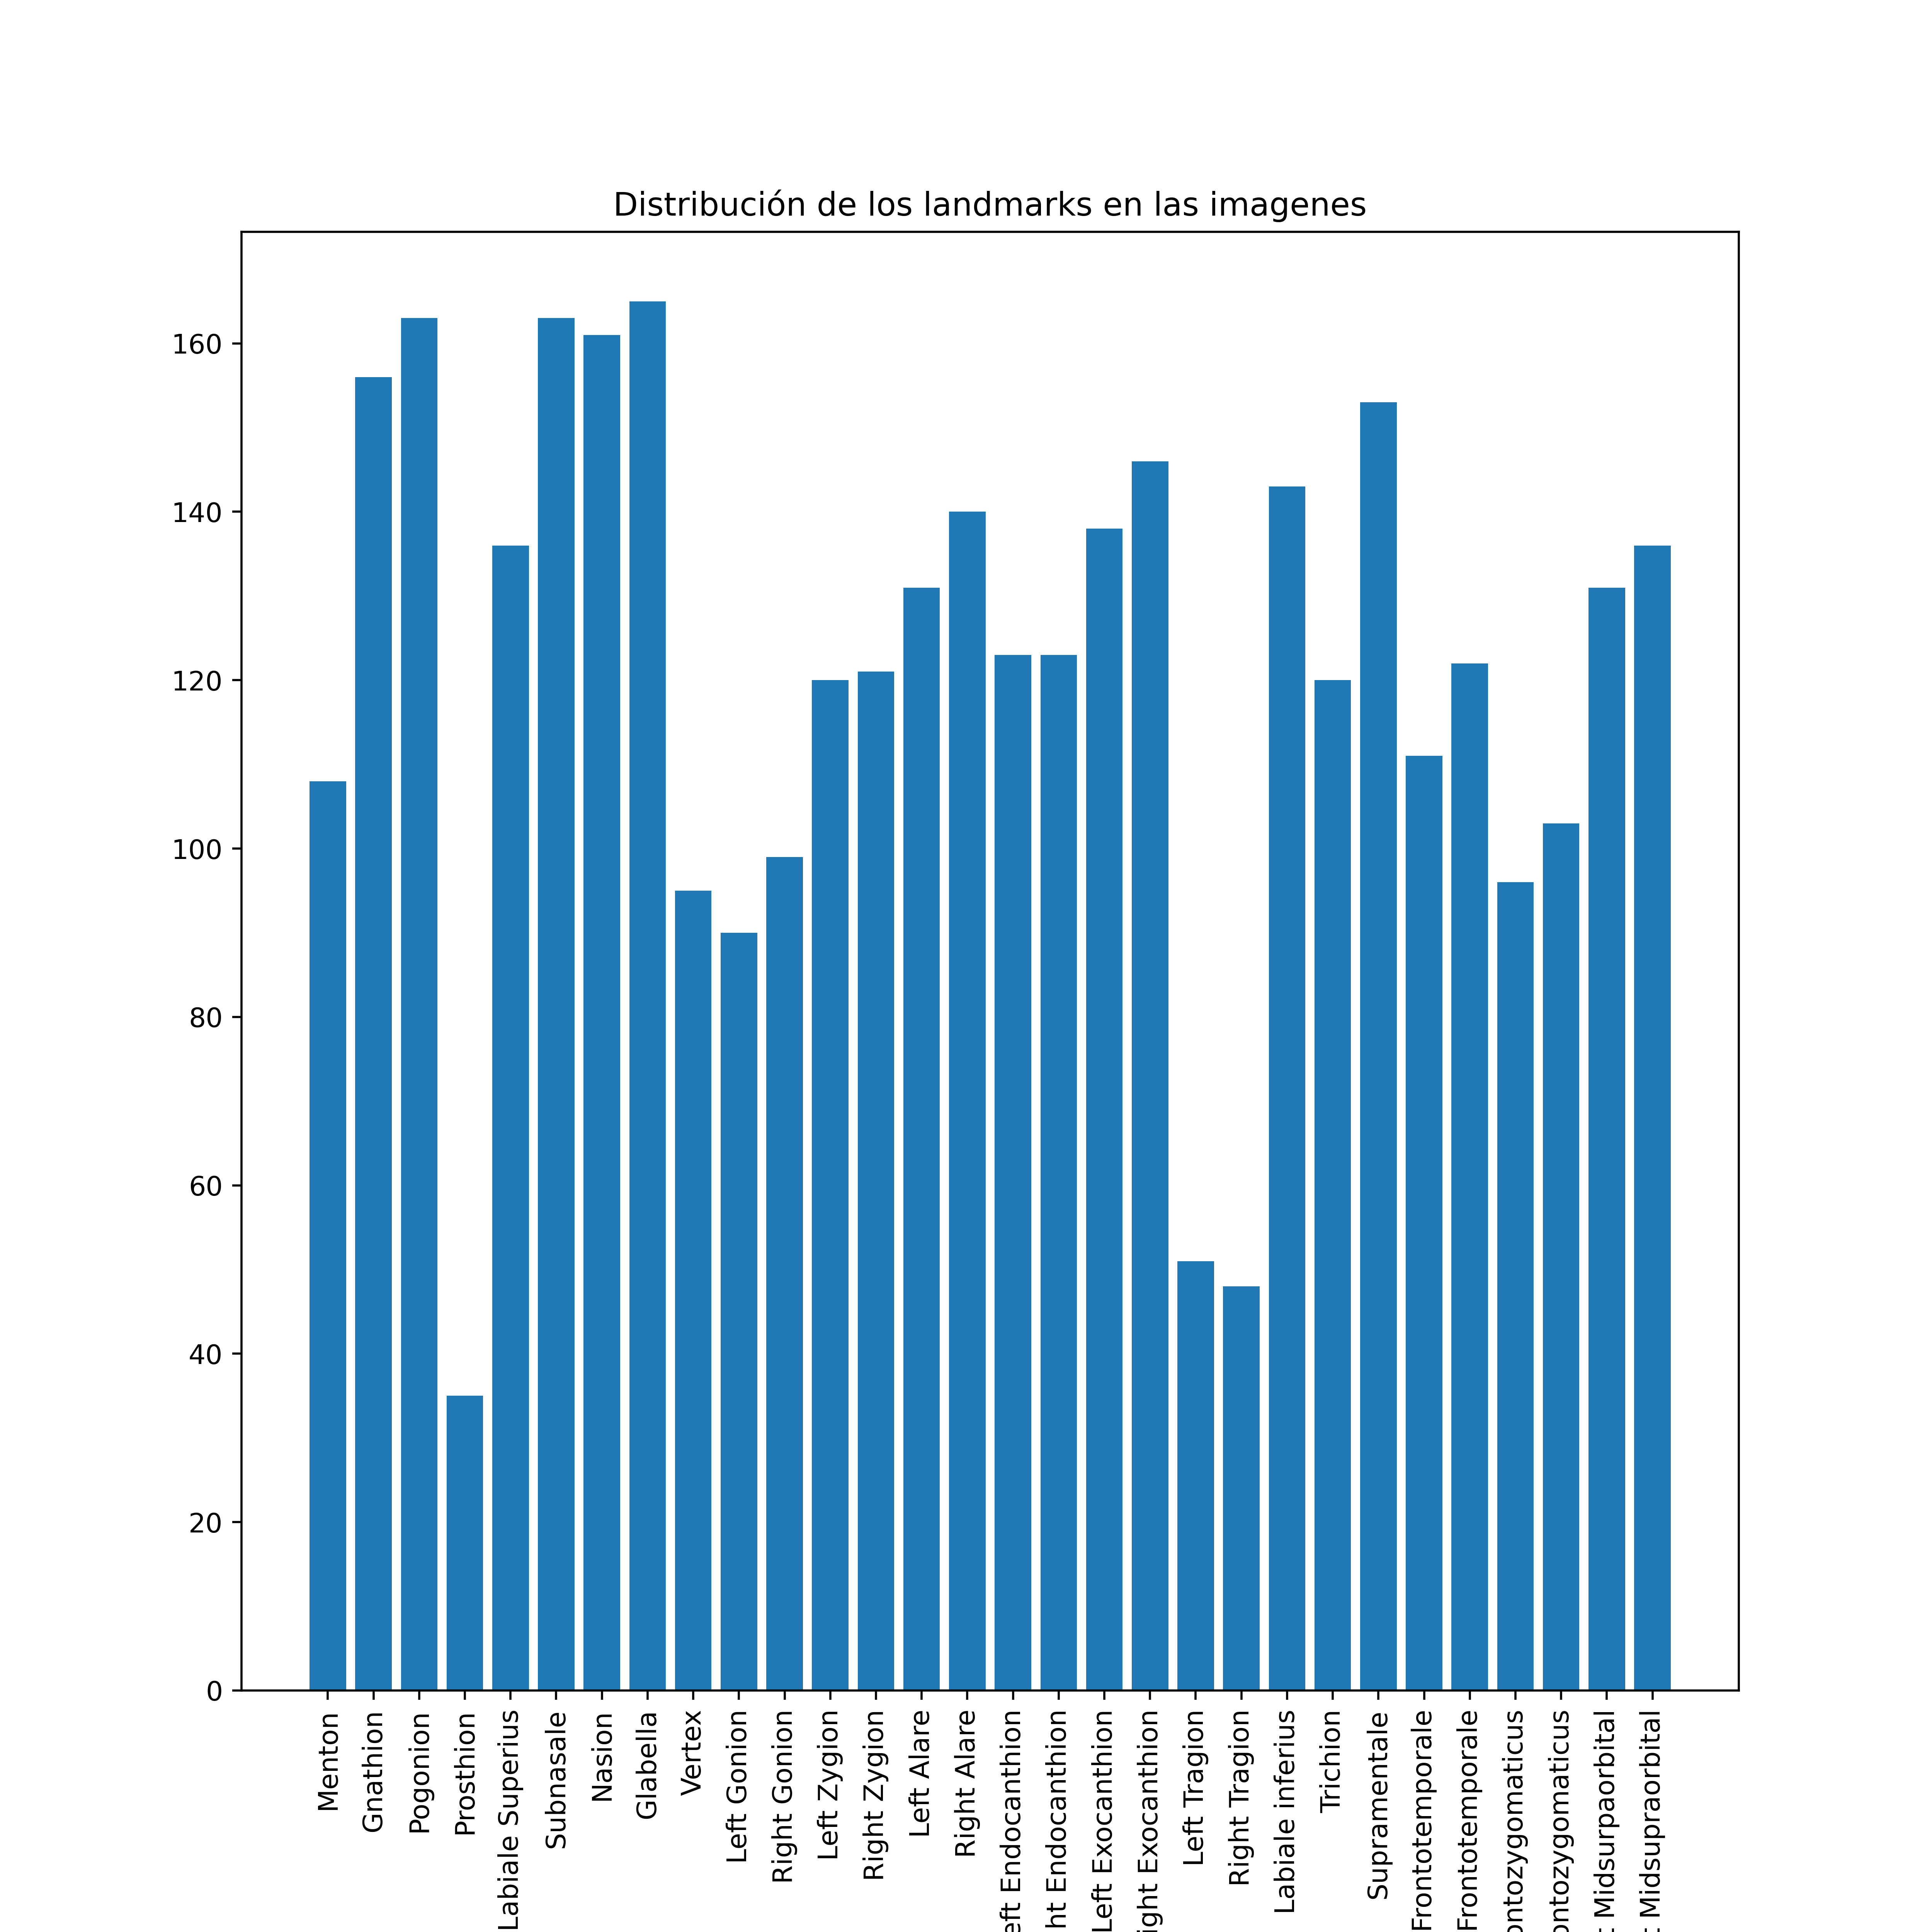
\includegraphics[width=0.7\textwidth]{img/distribucion_landmarks_imagenes.png}
                \caption{Histograma con la aparición de cada tipo de landmark en las imágenes del dataset.}
                \label{fig:Histograma}
            \end{figure}

    \section{Red empleada: 3FabRec}
        \noindent La red empleada para la resolución del problema es la desarrollada por \textbf{Bjorn Browatzki et al} en $2020$ \cite{browatzki20203fabrec} denominada \textbf{3FabRec}.La red en cuestión es un \textbf{Adversarial Autoencoder} que ha sido modificado para poder predecir landmarks incluyendo unas capas intermedias denominadas \textit{Interleaved Transfer Layer} en la etapa de reconstrucción.
         

        \medskip

        \noindent Aplica un método \textit{semi-supervisado} en el cual:
        
        \begin{itemize}
            \item Hay una primera fase de \textbf{aprendizaje no supervisado} dónde se pretende adquirir conocimiento implícito sobre la estructura facial contenida en grandes conjuntos de imágenes de rostros de personas en diversas posiciones, iluminación y etnia. Para ello se codifica todo este conocimiento implícito en un vector de un espacio latente de baja dimensionalidad para posteriormente reconstruir la imagen. Este proceso se hace íntegramente en el \textit{Adversarial Autoencoder}.
            \item Posteriormente, en una segunda fase de \textbf{aprendizaje supervisado}, se entrena la red con un conjunto de imágenes etiquetadas con landmarks faciales que la red tratará de predecir. Para ello se intercalan entre las capas del generador capas de convolución encargadas de reconstruir los mapas de calor de cada landmark junto con la reconstrucción del rostro del paso previo.
            \item Finalmente, se puede incluir una tercera fase de \textit{finetuning} en la cual se entrena el Encoder para mejorar el rendimiento en la predicción de landmarks.
        \end{itemize} 

        \begin{figure}[!h]
            \centering
            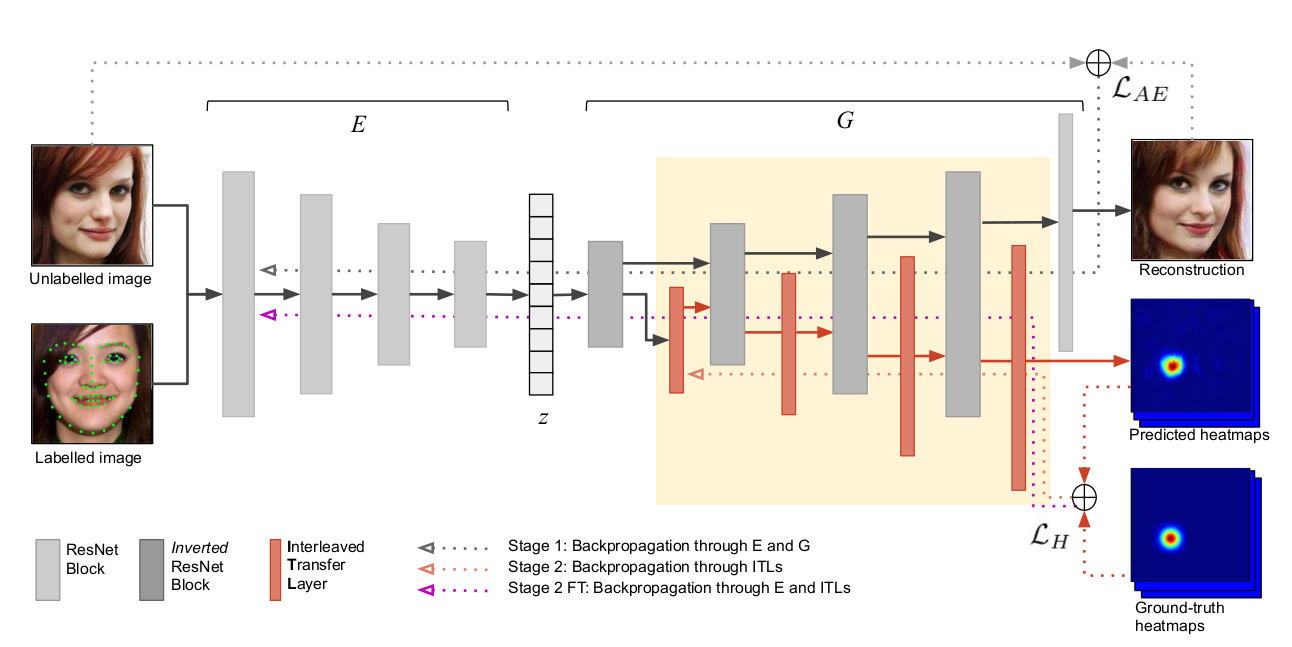
\includegraphics[width=0.7\textwidth]{img/3fabrec_arquitectura.png}
            \caption{Imagen resumen del framework 3FabRec. En ella podemos ver la estructura del \textit{Adversarial Autoencoder}, dividido en un Encoder (región bajo la \textit{E}) y un Generator (región bajo la \textit{G}) }
            \label{fig:3FabRec Resumen}
        \end{figure}

        \subsection{Arquitectura Adversarial Autoencoder}
            \noindent Para la construcción del \textit{Adversarial Autoencoder} emplean:
            
            \begin{itemize}
                \item \textbf{Encoder}: emplean una ResNet-$50$  hasta codificar la entrada en un vector de $99$ dimensiones. Está pensado para imágenes de res $256 \times 256 \times 3$, aunque se adapta también a imágenes de dimensiones $512 \times 512 \times 3$.
                \item \textbf{Decoder}: emplean la misma red ResNet-$50$ pero invertida.
            \end{itemize}

            \noindent Para una mejor comprensión he realizado unos diagramas con la herramienta \textit{diagrams.net}. En la \autoref{fig:bloque_encoder} podemos ver la estructura básica de los bloques de la ResNet-$50$.

            \begin{figure}[!h]
                \centering
                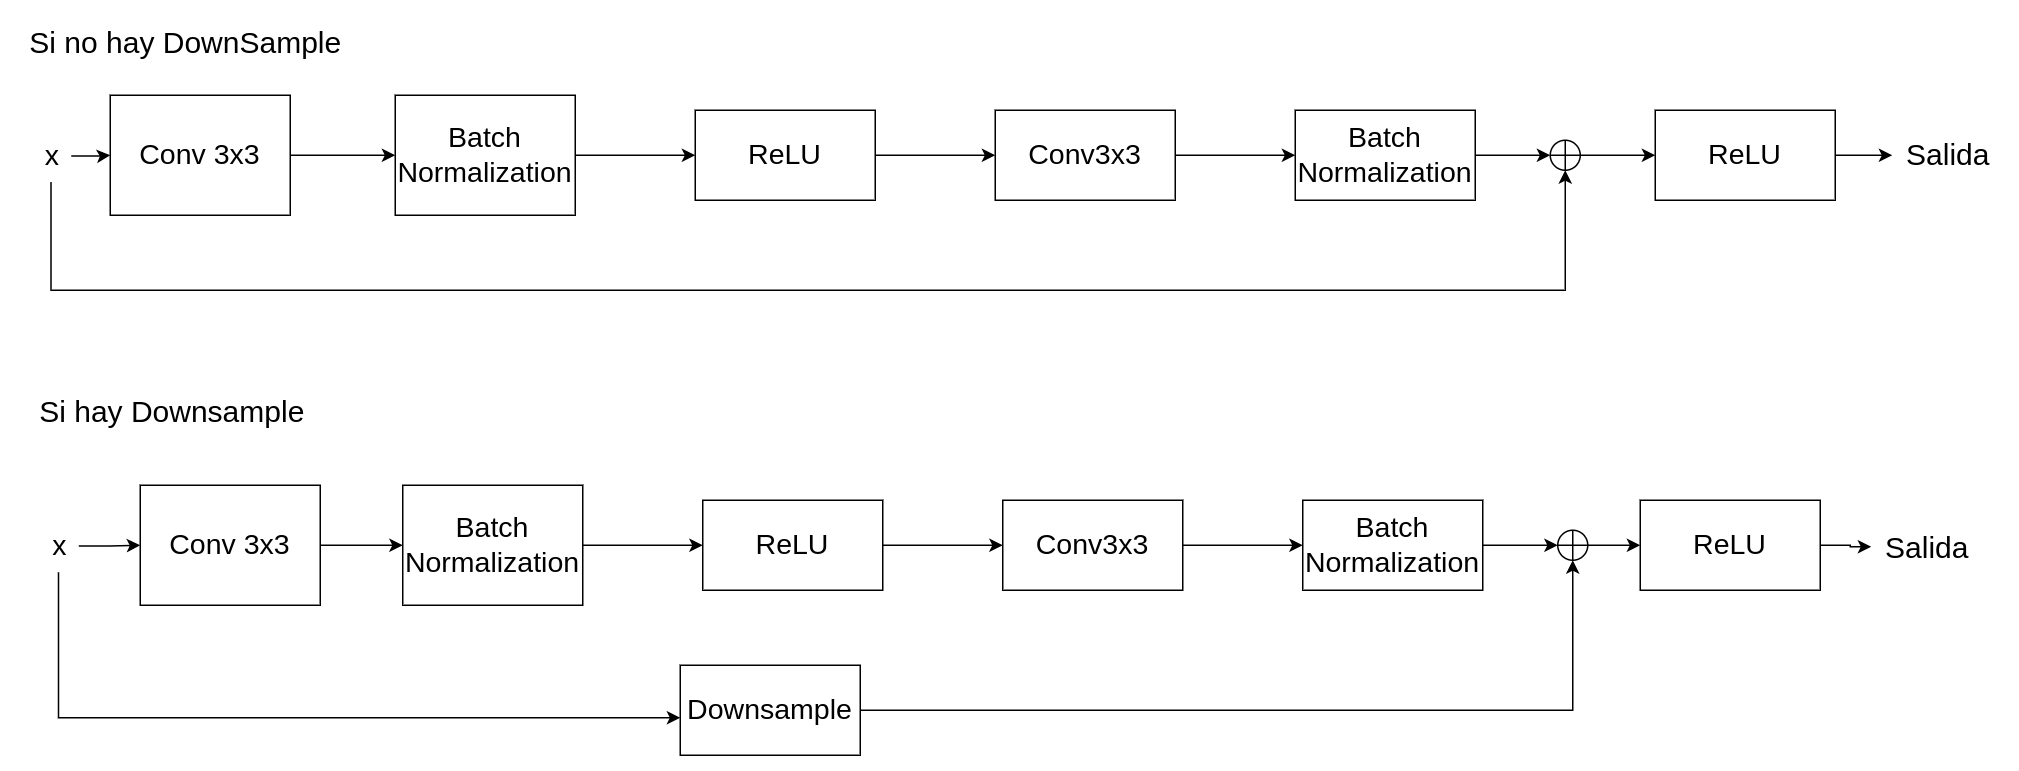
\includegraphics[width=0.7\textwidth]{img/bloque_basico_encoder.png}
                \caption{Bloques básicos que utilza la red ResNet-$50$ en sus capas. Se trata de una sucesión clásica de Convolución 3x3 + Batch Normalization + ReLU que se repite dos veces. En el primer caso los filtros de convolución no reducen las dimensiones del tensor añadiendo un padding de 1. En el segundo caso se reduce la dimensión del tensor a la mitad tras la primera convolución y se manteiene la dimensionalidad en la segunda. En el primer caso, la suma residual puede realizarse con el tensor x sin problema, en el segundo caso el tensor debe reducirse para que casen las dimensiones.}
                \label{fig:bloque_encoder}
            \end{figure}

            \medskip 

            \noindent Por otro lado en la \autoref{fig:Paso_encoder} podemos ver el paso de una imagen de entrada de tres canales y resolución $256 \times 256$ por el encoder.

            \begin{figure}[!h]
                \centering
                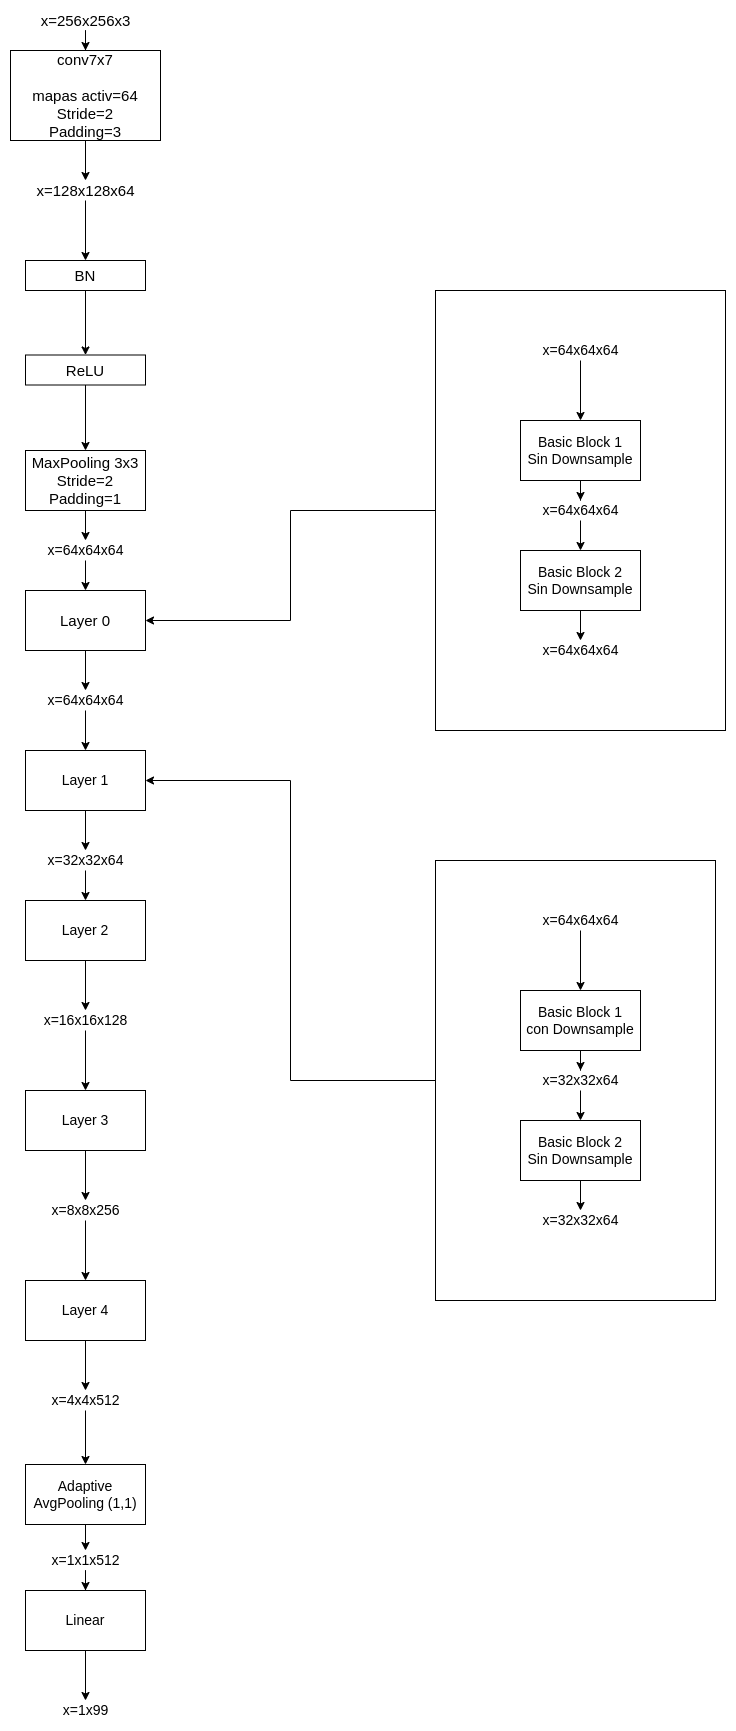
\includegraphics[width=0.7\textwidth]{img/3FabRec-Page-2.drawio.png}
                \caption{Ejemplo de paso de una imagen a través del Encoder. Cabe destacar que a partir de la Layer 1, todos los bloques tienen downsample.}
                \label{fig:Paso_encoder}
            \end{figure}

            \medskip

            \noindent Por otro lado en la \autoref{fig:Bloque_Decoder} podemos ver la estructura básica de un bloque en el Generador \textit{Inverse ResNet}, y un ejemplo del paso de un vector por el generador podemos verlo en la \autoref{fig:Paso_Generator}

            \begin{figure}[!h]
                \centering
                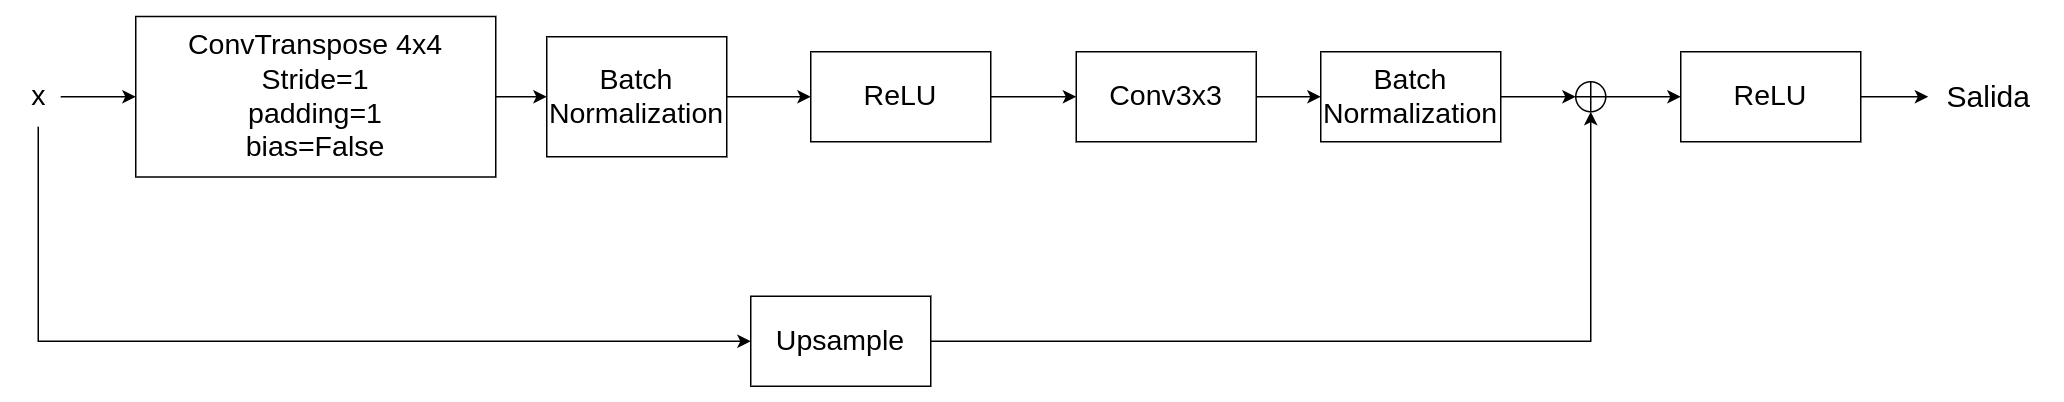
\includegraphics[width=0.7\textwidth]{img/bloque_invresnet.png}
                \caption{En primer lugar se aplica una convolución transpuesta que duplica las dimensiones del tensor de entrada y tras esto se sigue la misma estructura que en el bloque básico de la ResNet-$50$, la segunda convolución $3\times 3$ mantiene las dimensiones. Como consecuencia, para sumar el tensor de entrada con la salida del bloque se aumentan las dimensiones de este.}
                \label{fig:Bloque_Decoder}
            \end{figure}

            \begin{figure}[!h]
                \centering
                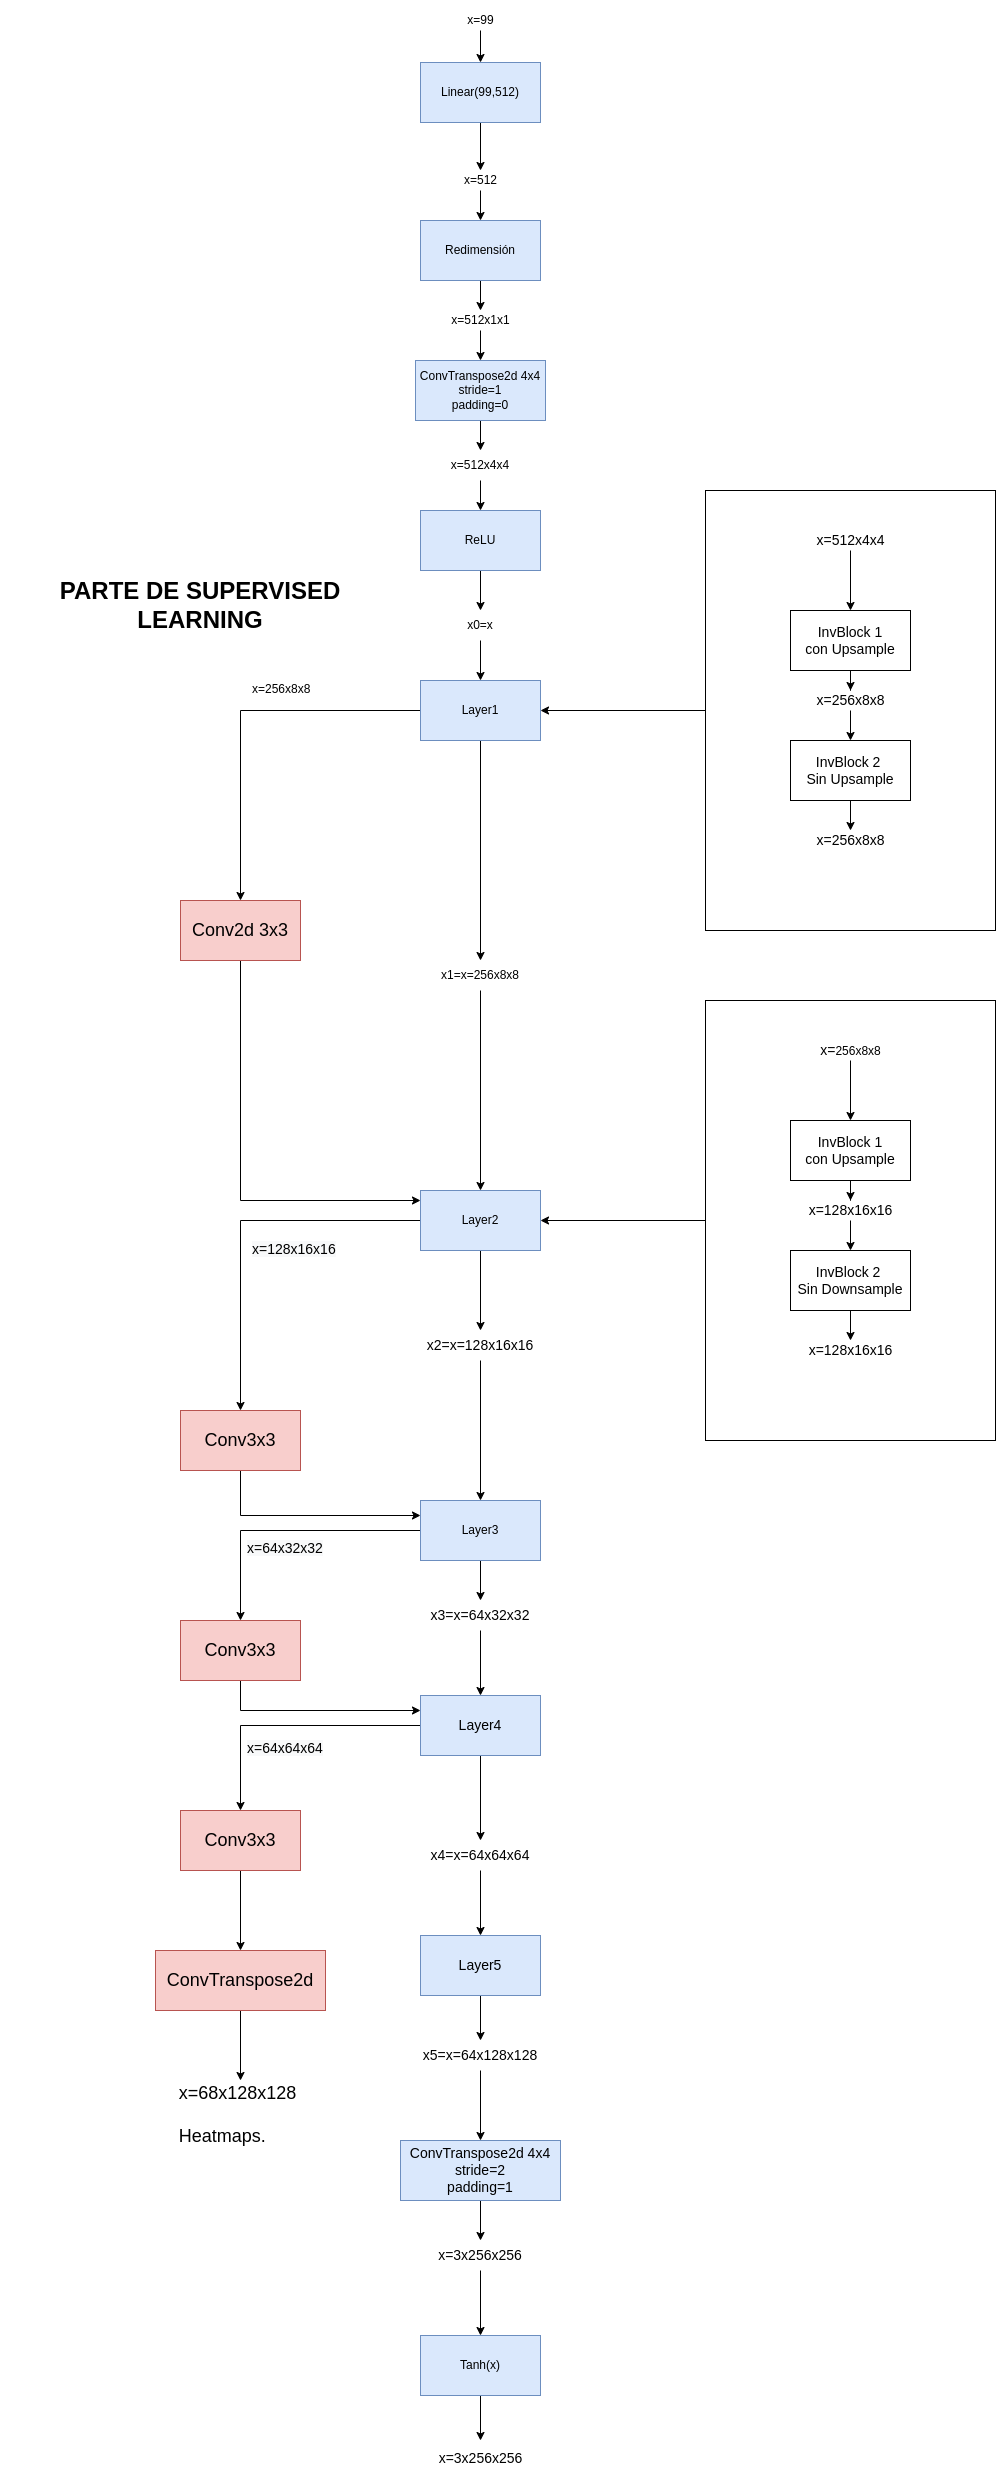
\includegraphics[width=0.5\textwidth]{img/paso_generator.png}
                \caption{Ejemplo del paso de un vector de $99$ dimensiones por el generador hasta reconstruirse la imagen de dimensiones $256 \times 256 \times 3$. La parte correspondiente al aprendizaje supervisado es la de los cuadrados azules, los cuadrados rojos corresponden a las \textit{ITLS} de la parte supervisada que se intercalan entre cada dos capas y dan como resultado los mapas de calor de los landmarks predichos.}
                \label{fig:Paso_Generator}
            \end{figure}

            \noindent Finalmente, para definir el autoencoder necesitamos un Discriminador que procure que los vectores del espacio vectorial latente sigan una determinada distribución que se trata de una normal multivariante estándar al que vamos a añadirle un segundo discriminador propio de las \textbf{GAN} que nos dirá si la imagen reconstruida procede de la distribución que siguen los píxeles de la imagen de inicio. En la \autoref{fig:DGaussian} las redes neuronales que definen ambos discriminadores.

            \begin{figure}[!h]
                \centering
                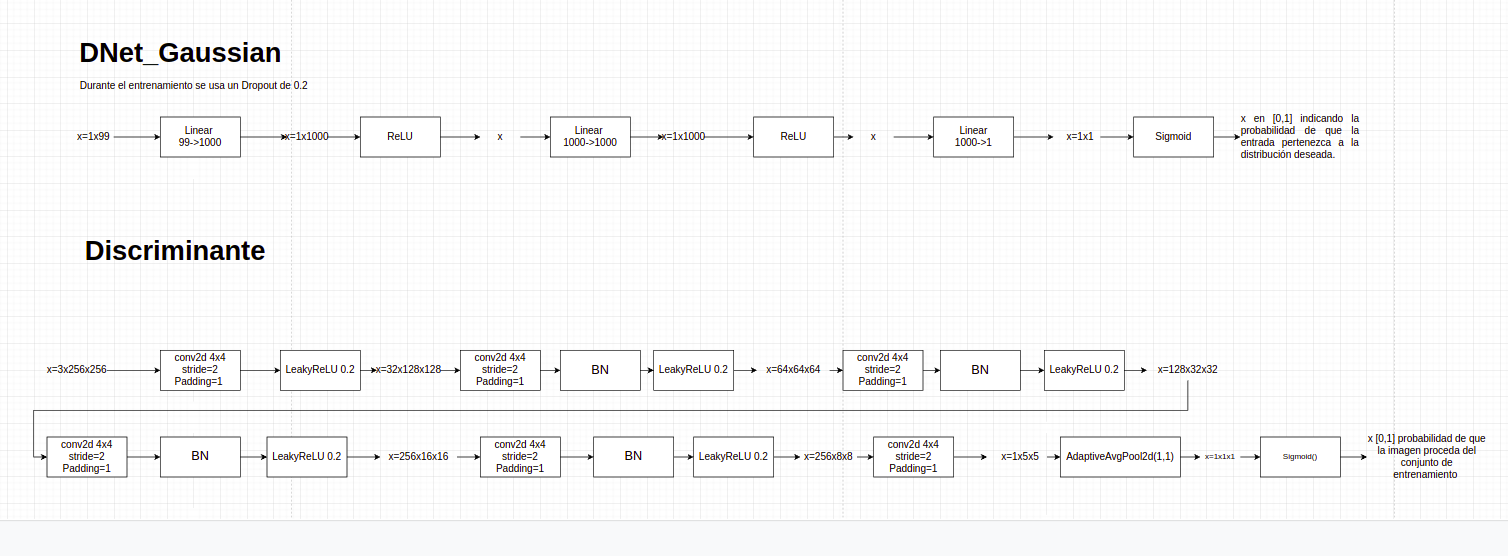
\includegraphics[width=0.99\textwidth]{img/DGaussian.png}
                \caption{En la imagen superior vemos el discriminante que se emplea para los vectores producidos por el Encoder y en la imagen inferior vemos el discriminante que se emplea para las imágenes generadas por el Generador. En ambos casos se da como salida un valor entre $0$ y $1$ que hace referencia a la probabilidad de pertenecer a la distribución deseada en el primer caso o a seguir la distribución de los píxeles de las imágenes en el segundo caso.}
                \label{fig:DGaussian}
            \end{figure}

        \subsection{Interleaved Transfer Layer (ITL)}
            
            \noindent Se tratan de simples capas convolucionales que se intercalan entre las capas del Generador. La última de estas capas proporciona como salida un conjunto de mapas de calor, uno por cada landmark predicho. Estos mapas de calor luego se emplean para representar en la imagen reconstruida los landmarks. La arquitectura de esta etapa podemos verla en la \autoref{fig:Paso_Generator}.

    \section{Metricas}
        
        \noindent A conitnuación mostraremos las métricas empleadas para estudiar la bondad de los resultados. Estas métricas también computan en la función de coste que explicaremos en la siguiente sección. 

        \subsection{SSIM}
            \noindent Se trata del \textit{structural similarity index} (SSIM) y da una medida de \textit{similaridad} entre dos imágenes \cite{wang2004image}, su expresión es la siguiente: 

            \begin{equation}
                SSIM(x,y)=[l(x,y)]^\alpha[c(x,y)]^{\beta}[s(x,y)]^{\gamma}
            \end{equation}

            \medskip

            \noindent Dónde $x,y$ son las dos imágenes que van a ser comparadas.

            \medskip

            \noindent La componente $c(x,y)$ hace referencia a la función de comparación del contraste de las dos imágenes y viene dada por la siguiente expresión: 

            \begin{equation}
                c(x,y)=\frac{2\sigma_x \sigma_y + C}{\sigma_x^2+ \sigma_y^2+C}
            \end{equation}

            \noindent Dónde $\sigma_x, \sigma_y$ hacen referencia a la desviación estándar de cada imagen.

            \medskip

            \noindent La componente $s(x,y)$ es la función de comparación estructural entre las dos imágenes y viene dada por la siguiente expresión:

            \begin{equation}
                s(x,y)=\frac{\sigma_{xy}+C/2}{\sigma_x \sigma_y +C/2}
            \end{equation}

            \noindent Dónde $\sigma_{xy}$ denota la covarianza.

            \medskip

            \noindent La componente $l(x,y)$ hace referencia a la \textit{luminosidad}, pero en el caso de 3FabRec se prescinde de esta componente, además los exponentes $\alpha, \beta , \gamma$ se igualan a $1$.

            \medskip

            \noindent Por otra parte siguen las indicaciones del paper original de SSIM que recomiendan usar estas comparaciones en regiones de la imagen y promediarlas en vez de aplicarlas sobre todo el conjunto de píxeles de la imagen, es por ello que la expresión final queda:

            \begin{equation}
                cs(x,y)=\frac{1}{|w|} \sum{c(x_w,y_w)s(x_w,y_w)}_w
            \end{equation}

            \noindent Dónde $w$ representa la ventana sobre la que se aplica la función y $|w|$ el total de ventanas. En nuestro caso se emplean ventanas de tamaño $31\times 31$.

        \subsection{Average pixel error}
            \noindent Se trata de la función de coste \textbf{L1} que se aplica a la imagen original y la reconstruida  y nos porporciona una medida del error de reconstrucción a nivel de pixel. Este error se obtiene para cada imagen y luego se devuelve el error promedio, por eso se denomina \textit{Average pixel error}.

        \subsection{MSE}
            \noindent Se trata de la función de coste \textbf{L2} usada para medir la diferencia entre los mapas de calor pertenecientes a los landmarks reales y los mapas de calor de los landmarks predichos.

    \section{Función de pérdida}

        \noindent Para el entrenamiento de la red se emplean dos funciones de pérdida, la primera que presentaremos se emplea en el entrenamiento del \textit{Adversarial Autoencoder}, en la parte no supervisada, y la segunda función de pérdida se empleará tanto en la parte de aprendizaje supervisado como en la de \textit{finetuning} del Encoder.

        \medskip

        \noindent La función de pérdida empleada para el entrenamiento del \textit{Adversarial Autoencoder} en la parte de aprendizaje no supervisado es la siguiente: 
        
        \begin{align*}
            \min_{E,G} \max_{D_z,D_x} & \mathcal{L}_{AE}(E,G,D_z,D_x) \\
            & \lambda_{rec} \mathcal{L}_{rec}(E,G) + \lambda_{cs}\mathcal{L}_{cs}(E,G) \\
            & + \lambda_{enc}\mathcal{L}_{enc}(E,D_z)+ \lambda_{adv} \mathcal{L}_{adv}(E,G,D_x)
        \end{align*}

    \section{Proceso de entrenamiento de la red}
\endinput
%------------------------------------------------------------------------------------
% FIN DEL CAPÍTULO. 
%------------------------------------------------------------------------------------

